% ==============================================================================
\chapter{Thin sensors studies}
\label{ch:ThinSensorsStudies}
%==============================================================================    

%% --------------------------------------------- %%
\section{Samples and sensors geometries}
Operating conditions for the Timepix3 readout ASICs:
\begin{itemize}
\item I\textsubscript{krum} DAC is set to 10.
\item TOT clock frequency: $40\,\megahertz$
\item VFBK: 150
\end{itemize}


 For most of the measurements, the DUT is perpendicular to the beam. A
 scan was done on the bias voltage and the threshold of the DUT. The
 bias scan allows to obtain the depletion voltage.

%% --------------------------------------------- %%
\section{Test-beam results for thin sensors}
\subsection{Bias scan}
\subsection{Threshold scan}
\subsection{Resolution vs. thickness}
\subsection{Efficiency vs. thickness}


\begin{figure}[htbp] \centering
  \begin{subfigure}[b]{0.45\textwidth}
    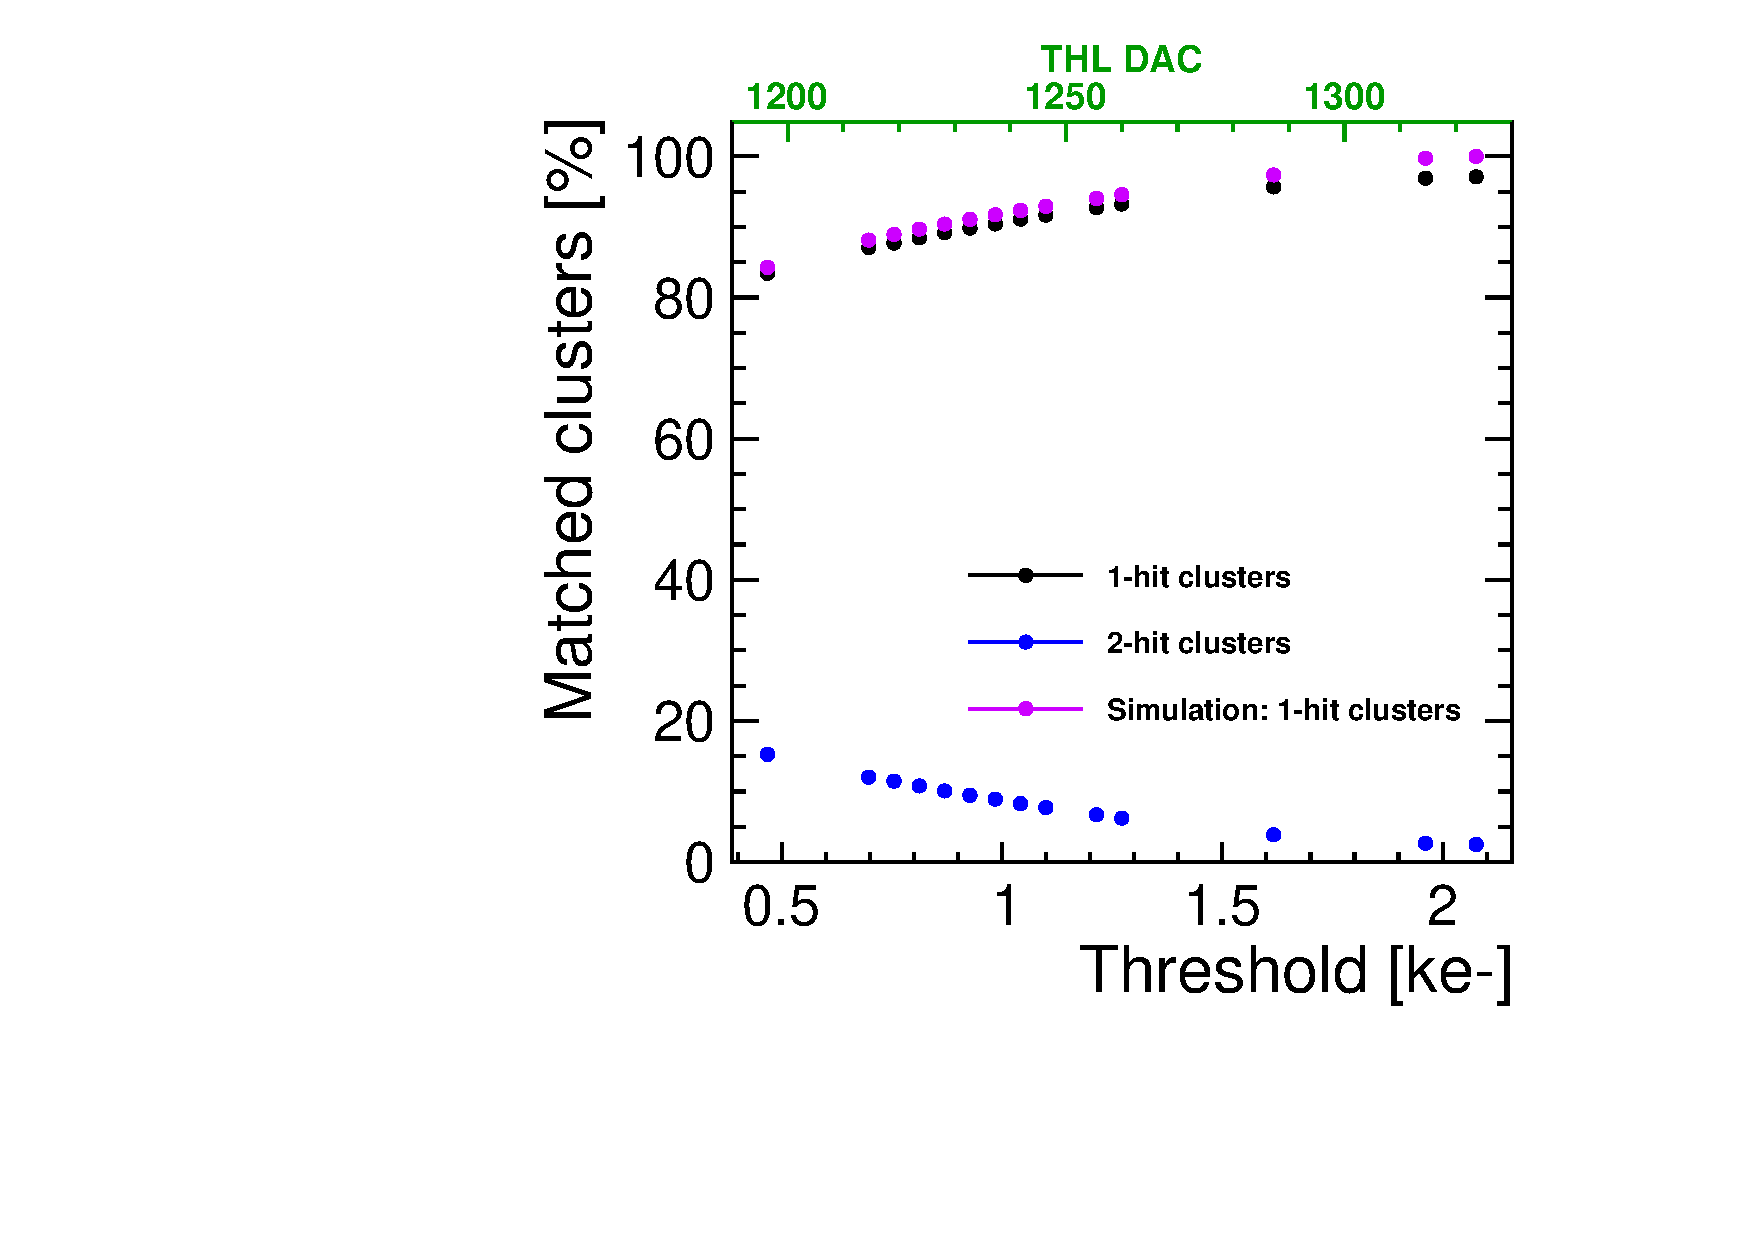
\includegraphics[width=\textwidth]{./figures/TestBeam/ThresholdScan_W0019_G07.pdf}
    \caption{}
  \end{subfigure} \hfill
  \begin{subfigure}[b]{0.45\textwidth}
    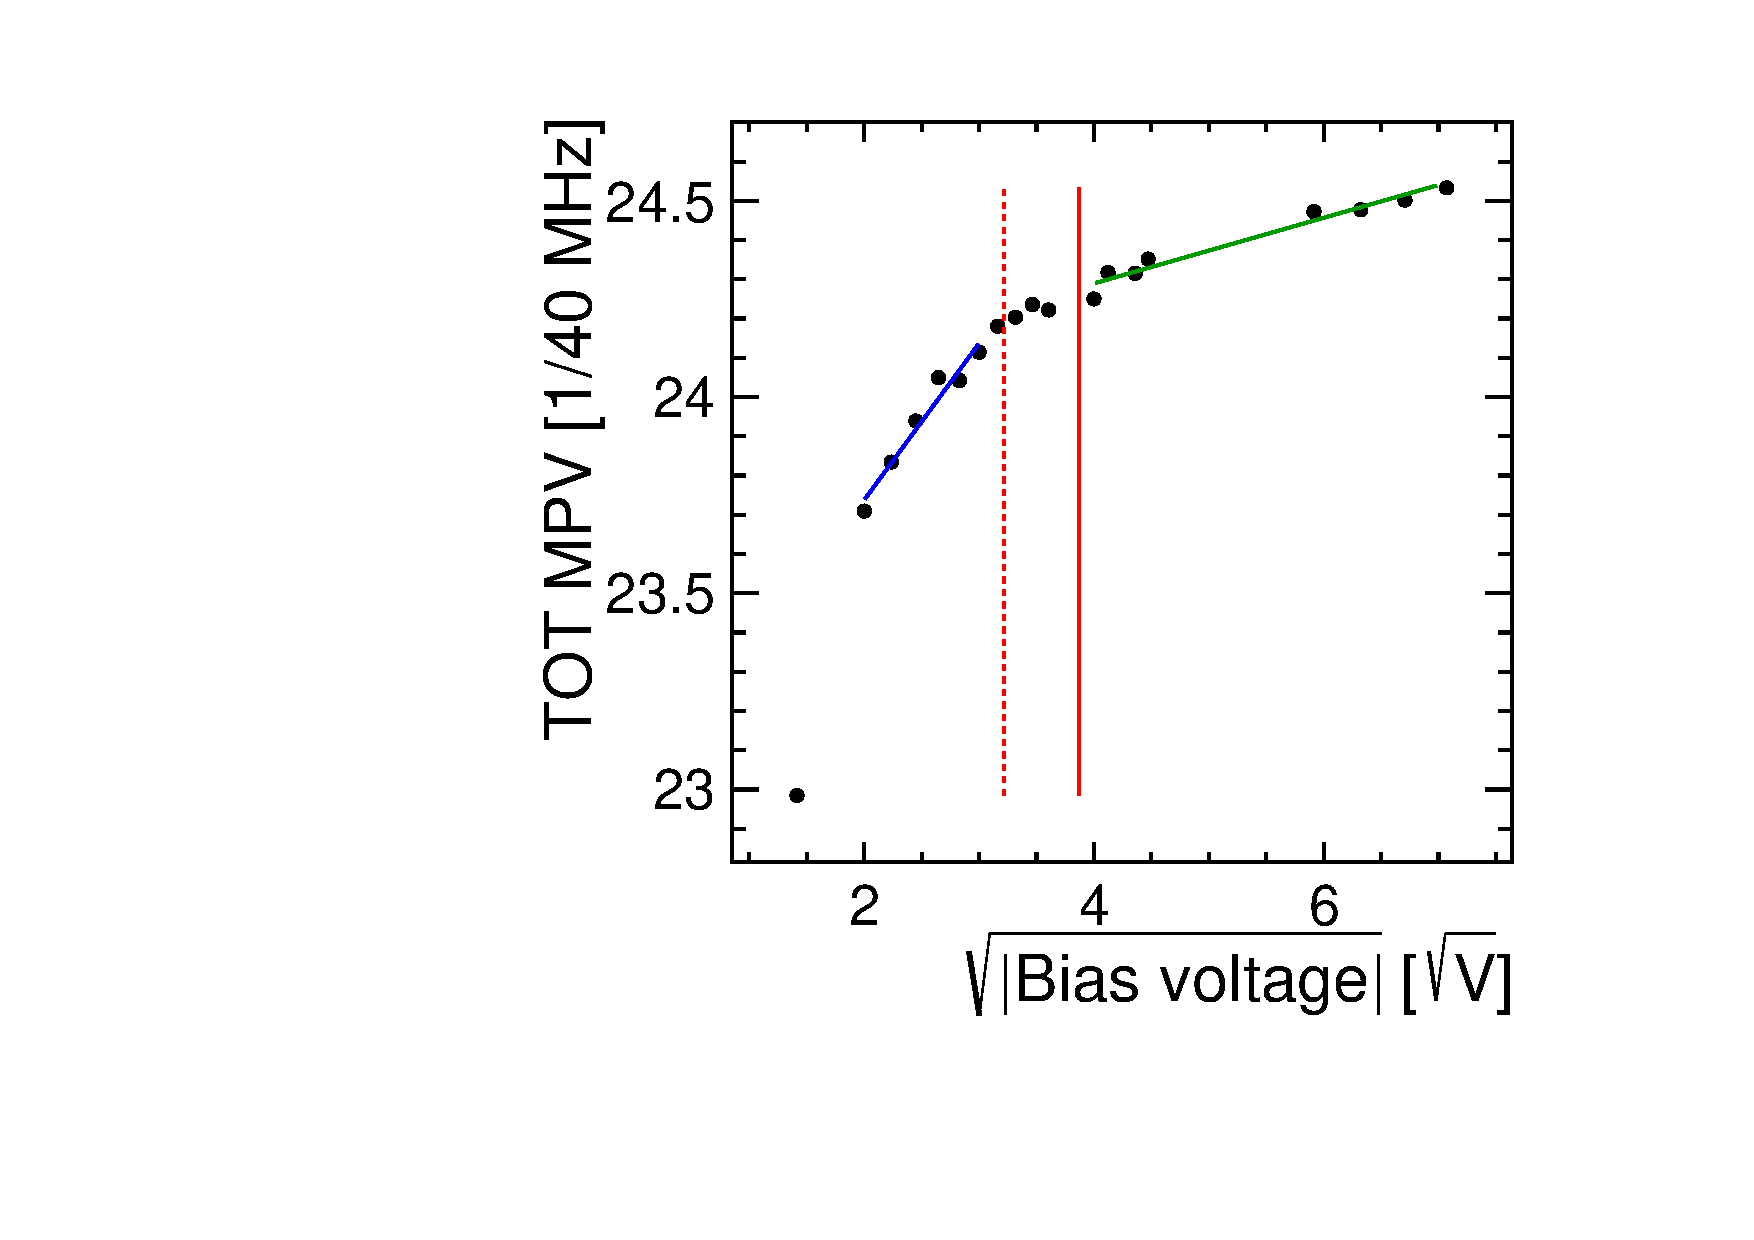
\includegraphics[width=\textwidth]{./figures/TestBeam/depletionVoltage_W0019_G07.pdf}
    \caption{}
  \end{subfigure}
  \caption{20-NGR (W19\_G7): bias and voltage scan.}
  \label{fig:Timepix3_THLscan_Vdep_G7}
\end{figure}

\begin{figure}[htbp] \centering
  \begin{subfigure}[b]{0.45\textwidth}
    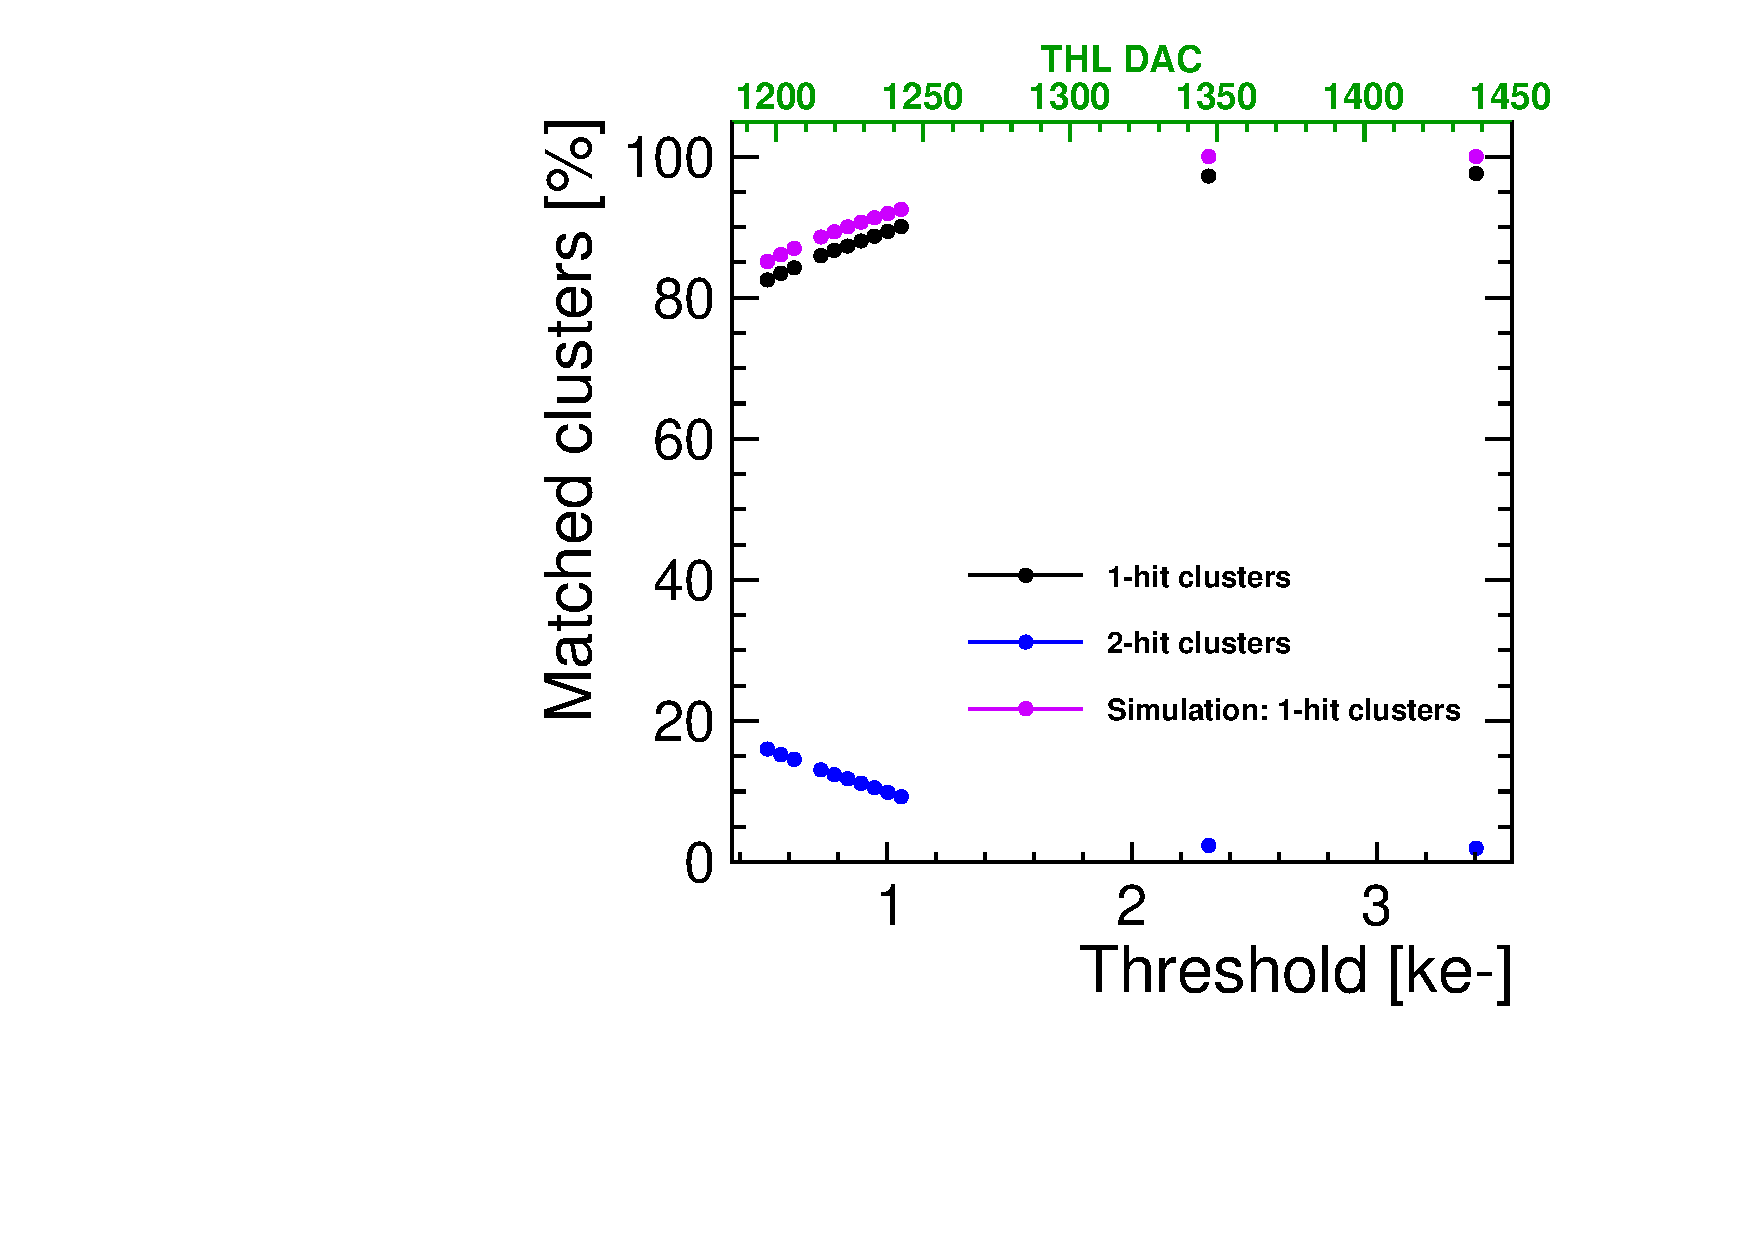
\includegraphics[width=\textwidth]{./figures/TestBeam/ThresholdScan_W0019_F07.pdf}
    \caption{}
  \end{subfigure} \hfill
  \begin{subfigure}[b]{0.45\textwidth}
    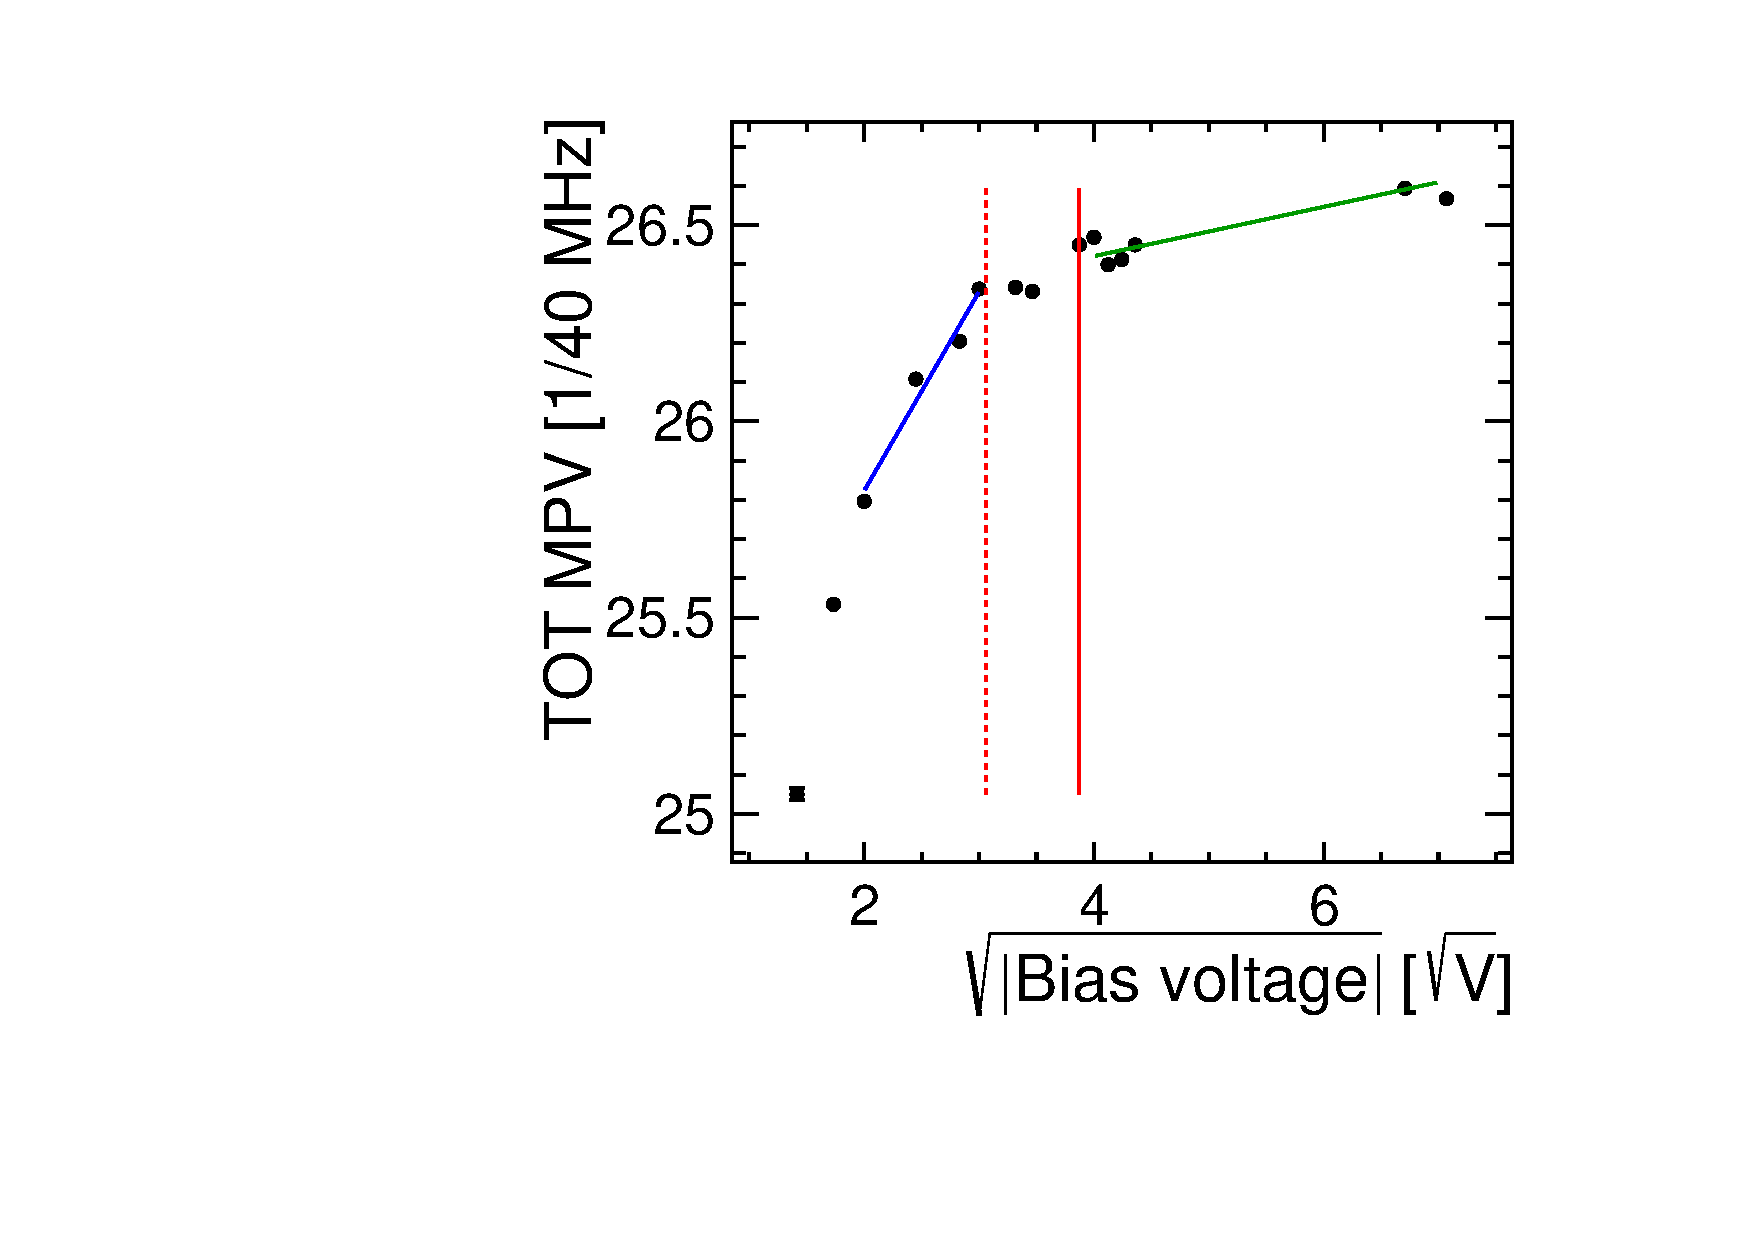
\includegraphics[width=\textwidth]{./figures/TestBeam/depletionVoltage_W0019_F07.pdf}
    \caption{}
  \end{subfigure}
  \caption{23-FGR (W19\_F7): bias and voltage scan.}
  \label{fig:Timepix3_THLscan_Vdep_F7}
\end{figure}

\begin{figure}[htbp] \centering
  \begin{subfigure}[b]{0.45\textwidth}
    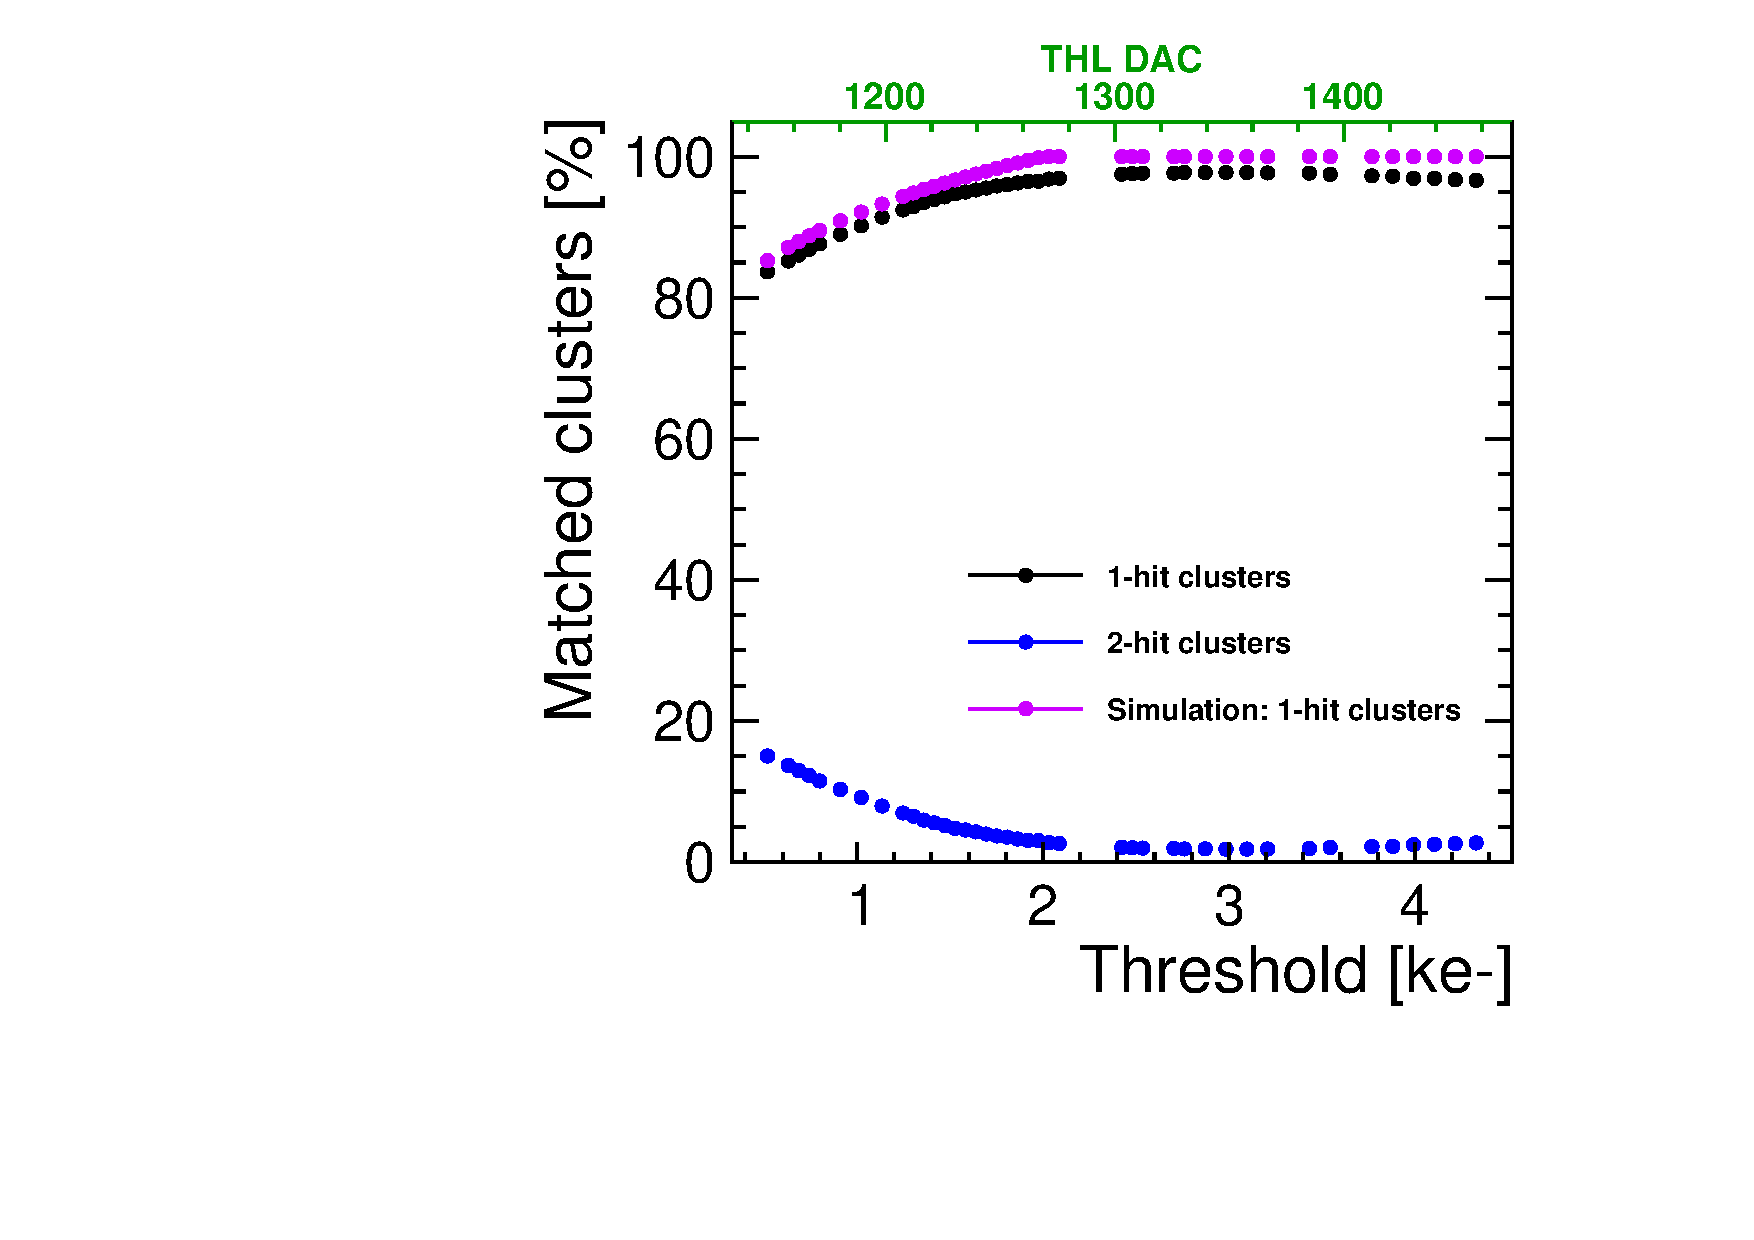
\includegraphics[width=\textwidth]{./figures/TestBeam/ThresholdScan_W0019_L08.pdf}
    \caption{}
  \end{subfigure} \hfill
  \begin{subfigure}[b]{0.45\textwidth}
    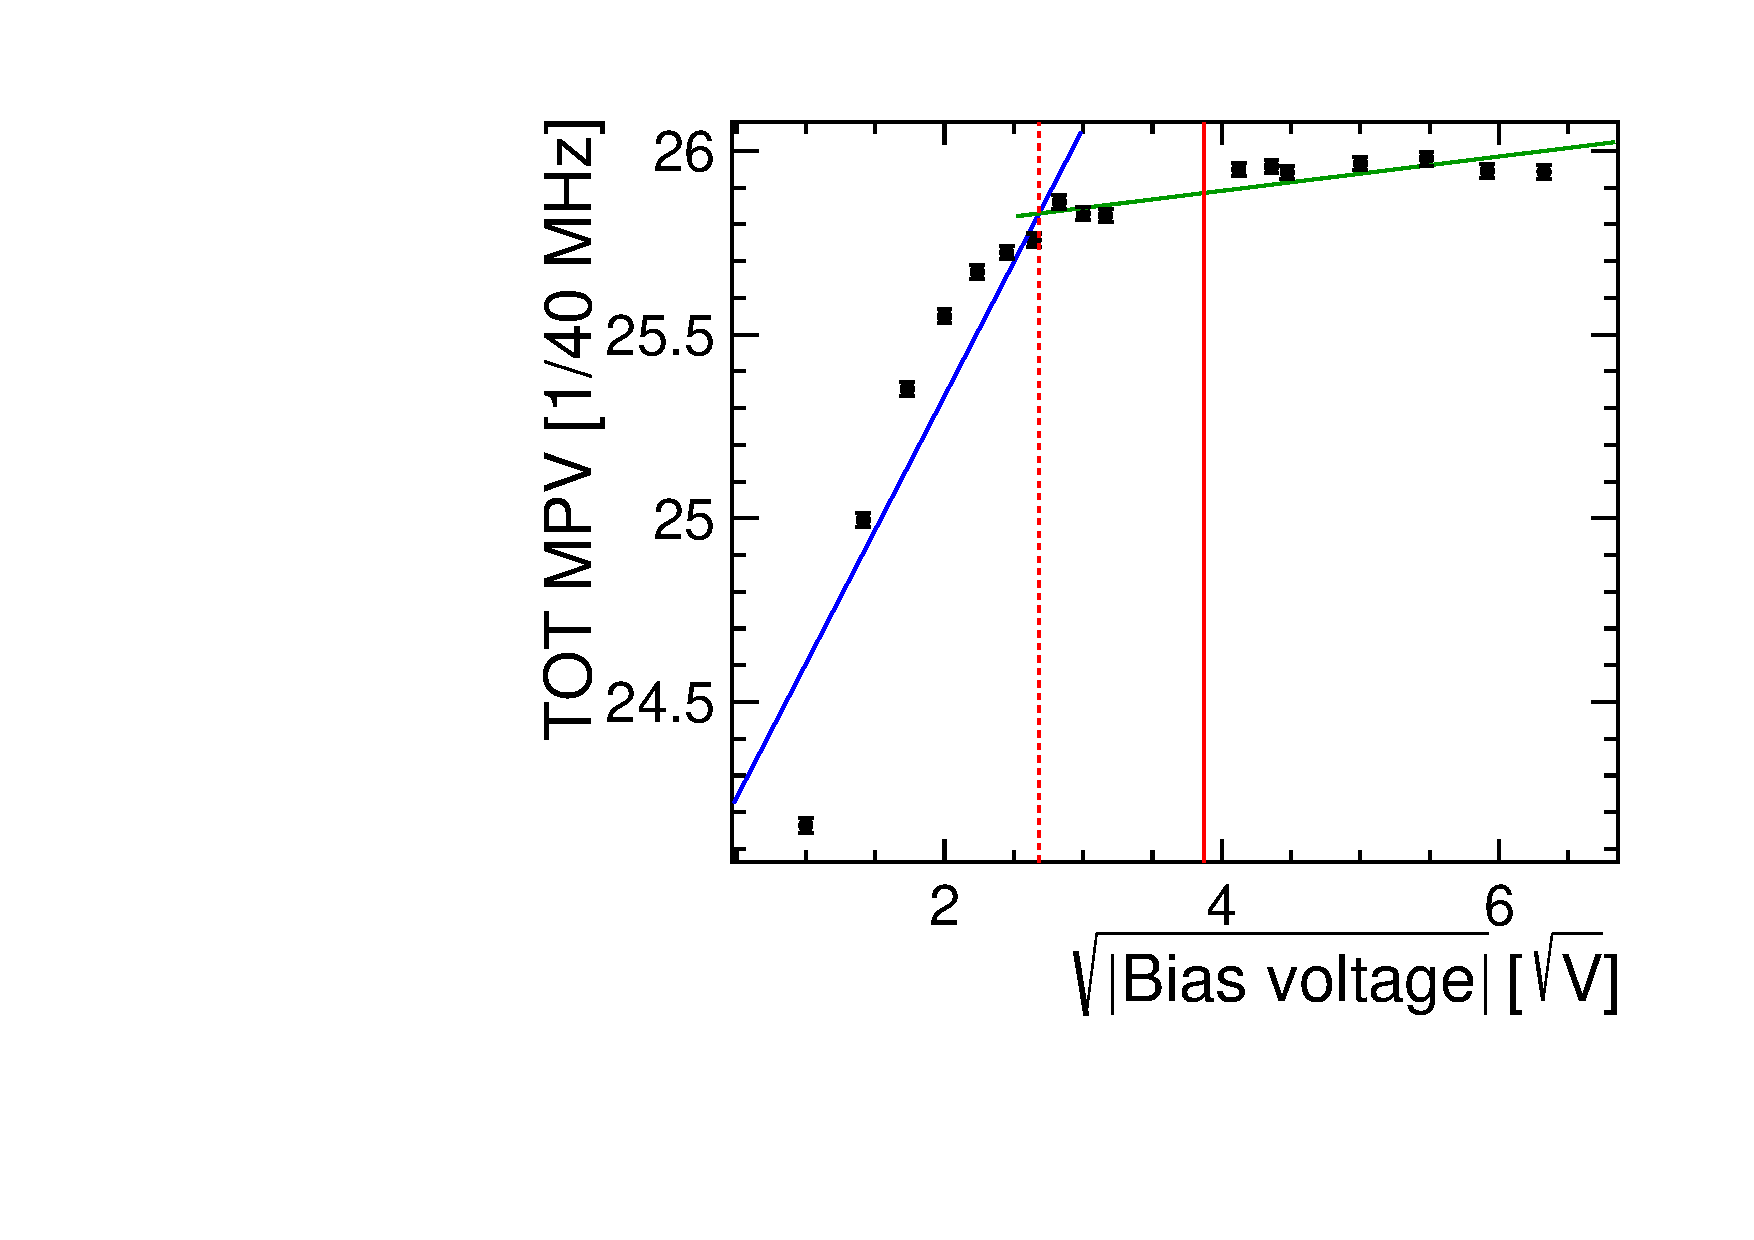
\includegraphics[width=\textwidth]{./figures/TestBeam/depletionVoltage_W0019_L08.pdf}
    \caption{}
  \end{subfigure}
  \caption{28-GNDGR (W19\_L8): bias and voltage scan.}
  \label{fig:Timepix3_THLscan_Vdep_L8}
\end{figure}


\begin{figure}[htbp] \centering
  \begin{subfigure}[b]{0.45\textwidth}
    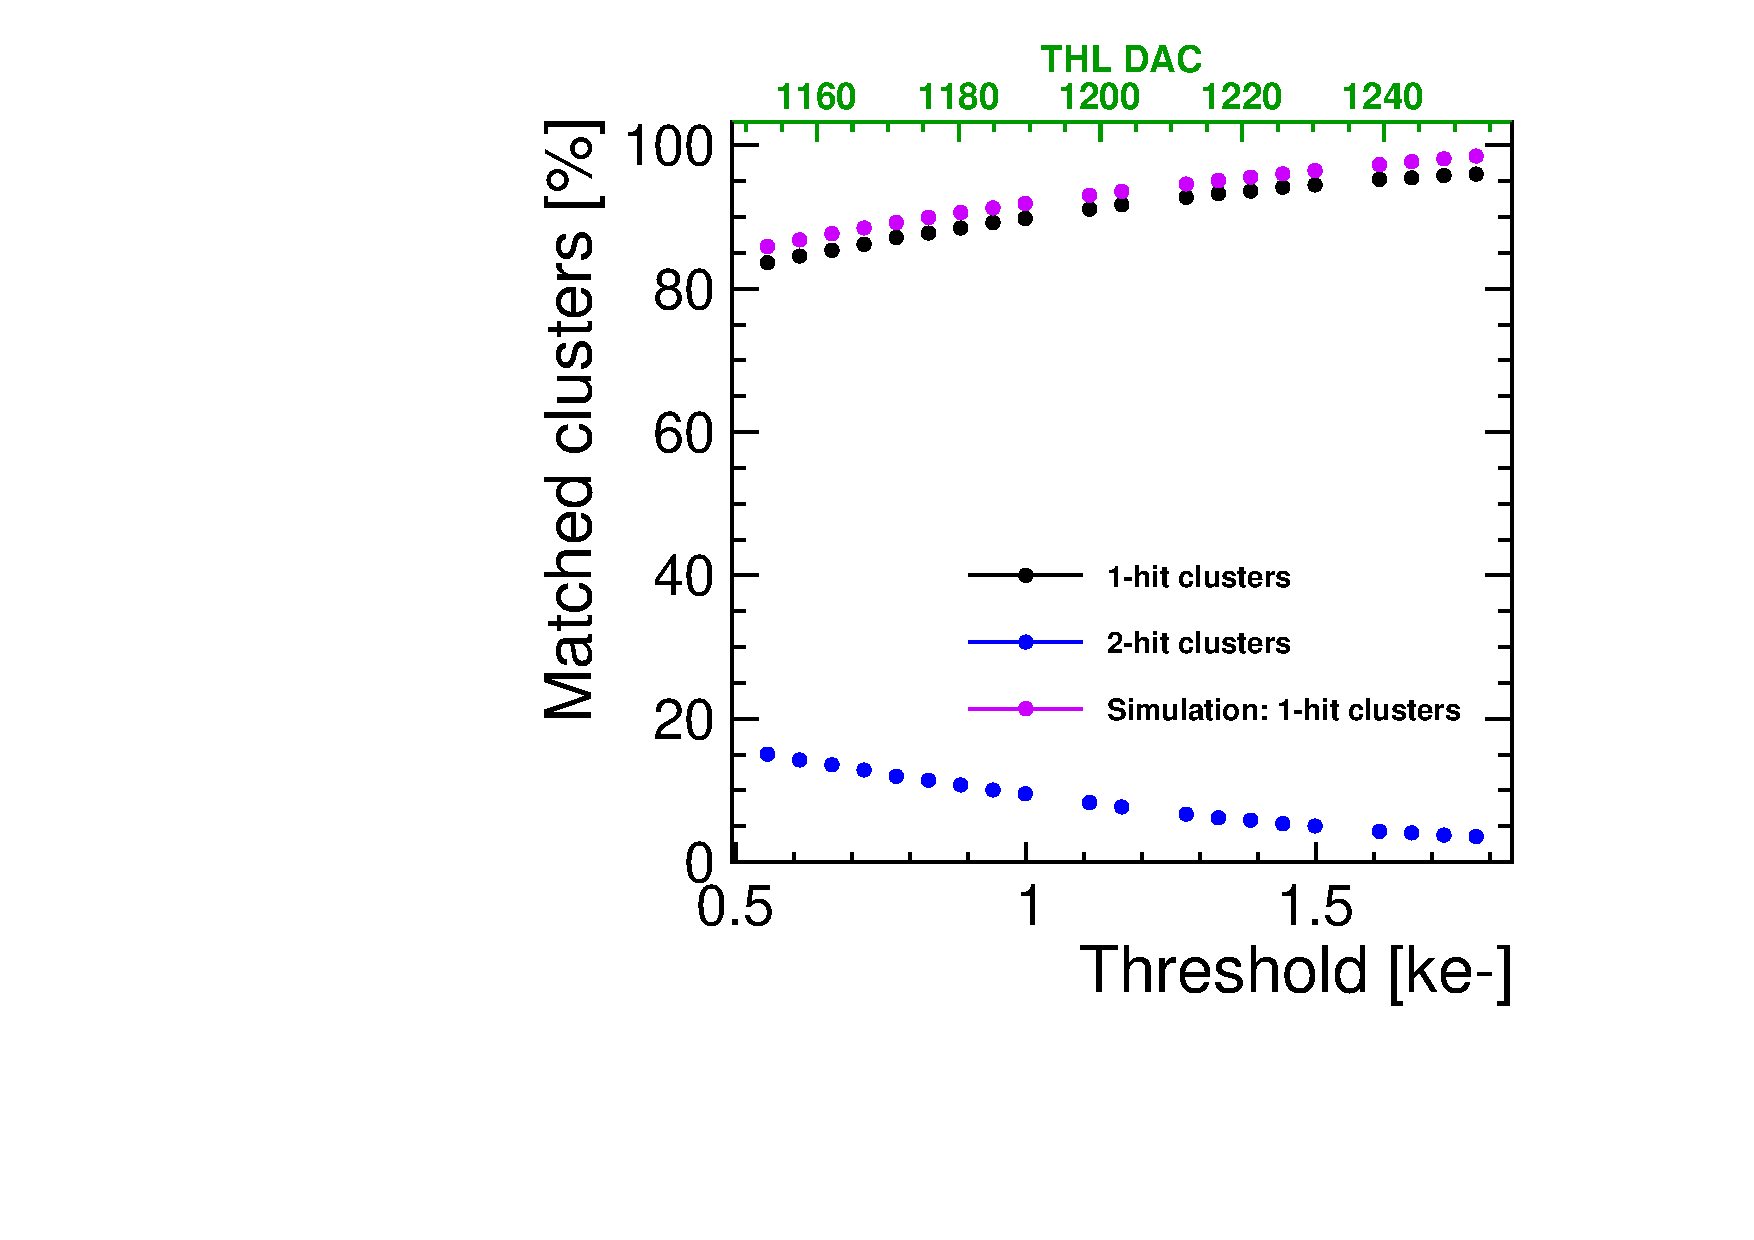
\includegraphics[width=\textwidth]{./figures/TestBeam/ThresholdScan_W0019_C07.pdf}
    \caption{}
  \end{subfigure} \hfill
  \begin{subfigure}[b]{0.45\textwidth}
    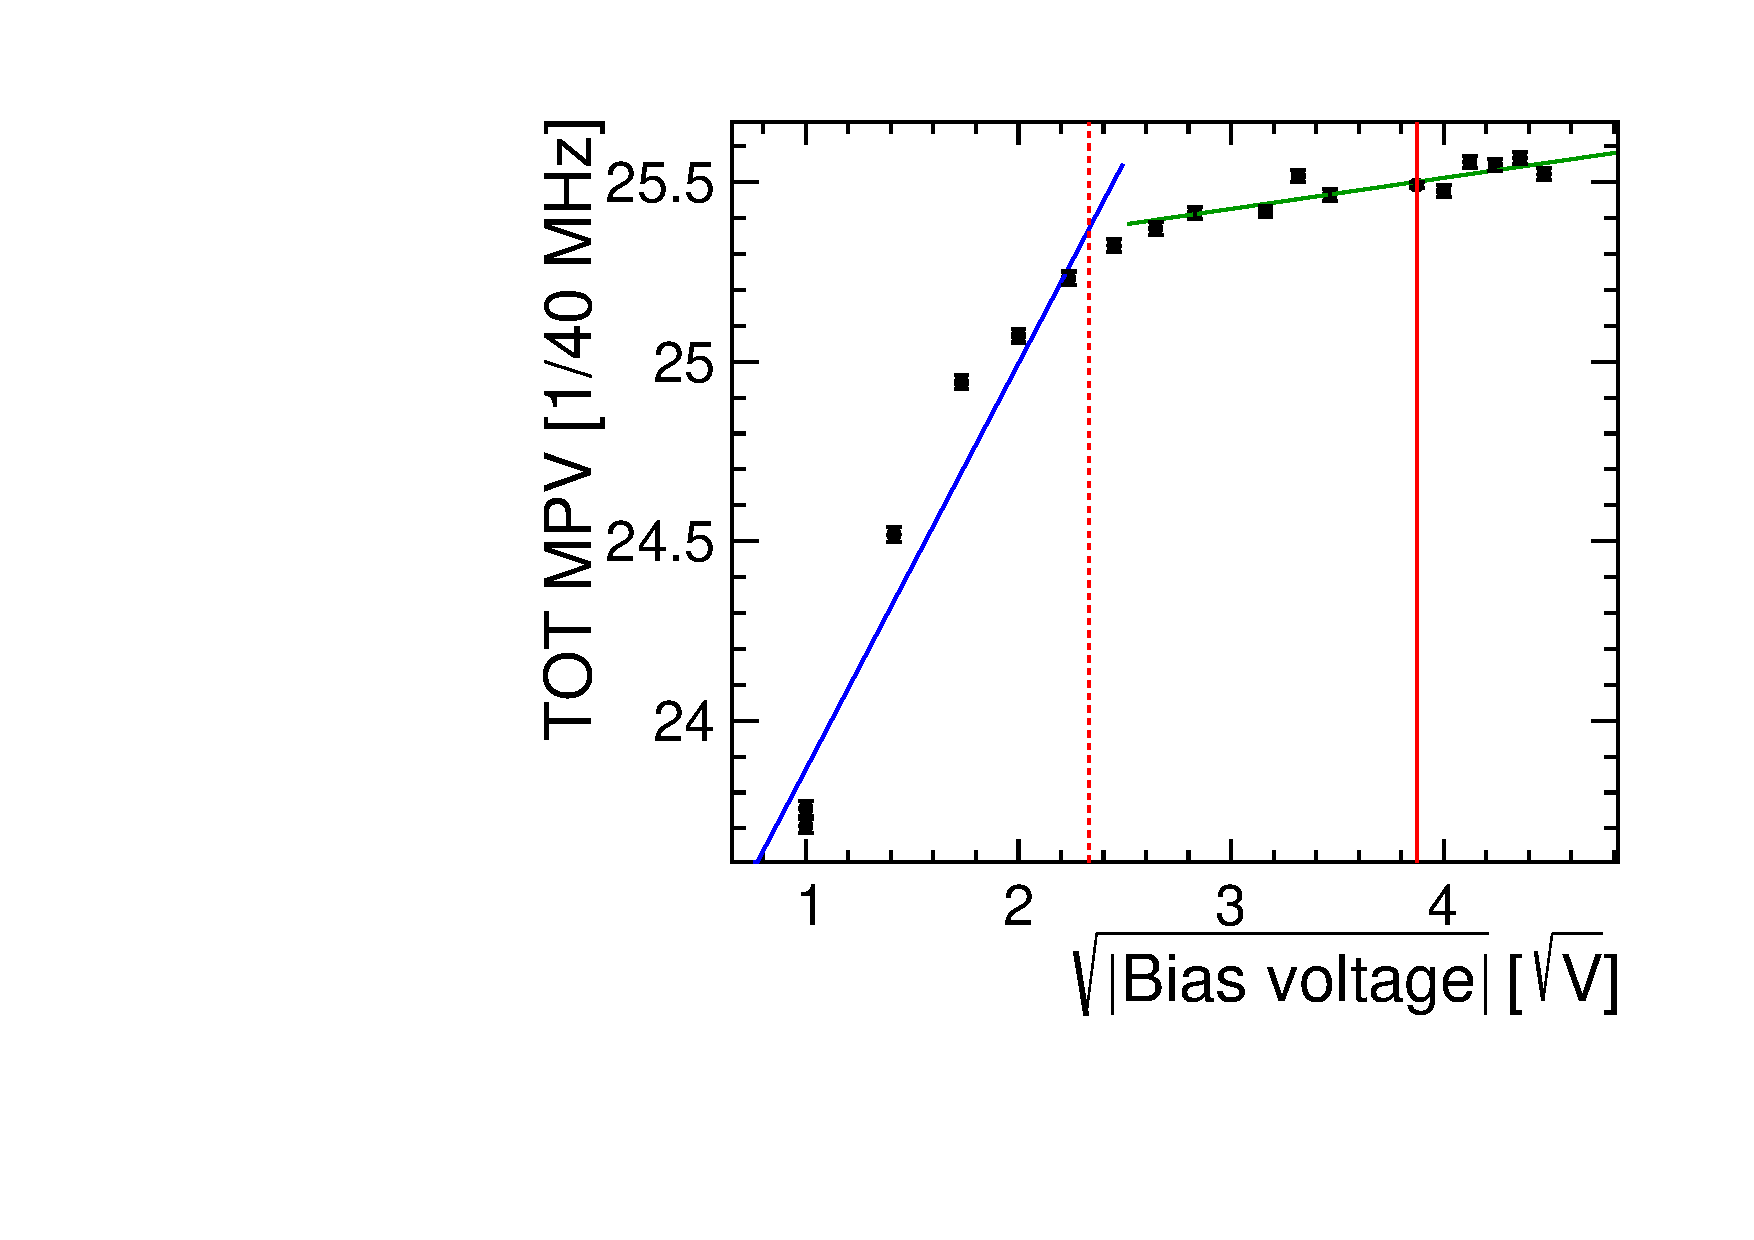
\includegraphics[width=\textwidth]{./figures/TestBeam/depletionVoltage_W0019_C07.pdf}
    \caption{}
  \end{subfigure}
  \caption{55-GNDGR (W19\_C7): bias and voltage scan.}
  \label{fig:Timepix3_THLscan_Vdep_C7}
\end{figure}

\begin{figure}[htbp] \centering
  \begin{subfigure}[b]{0.45\textwidth}
    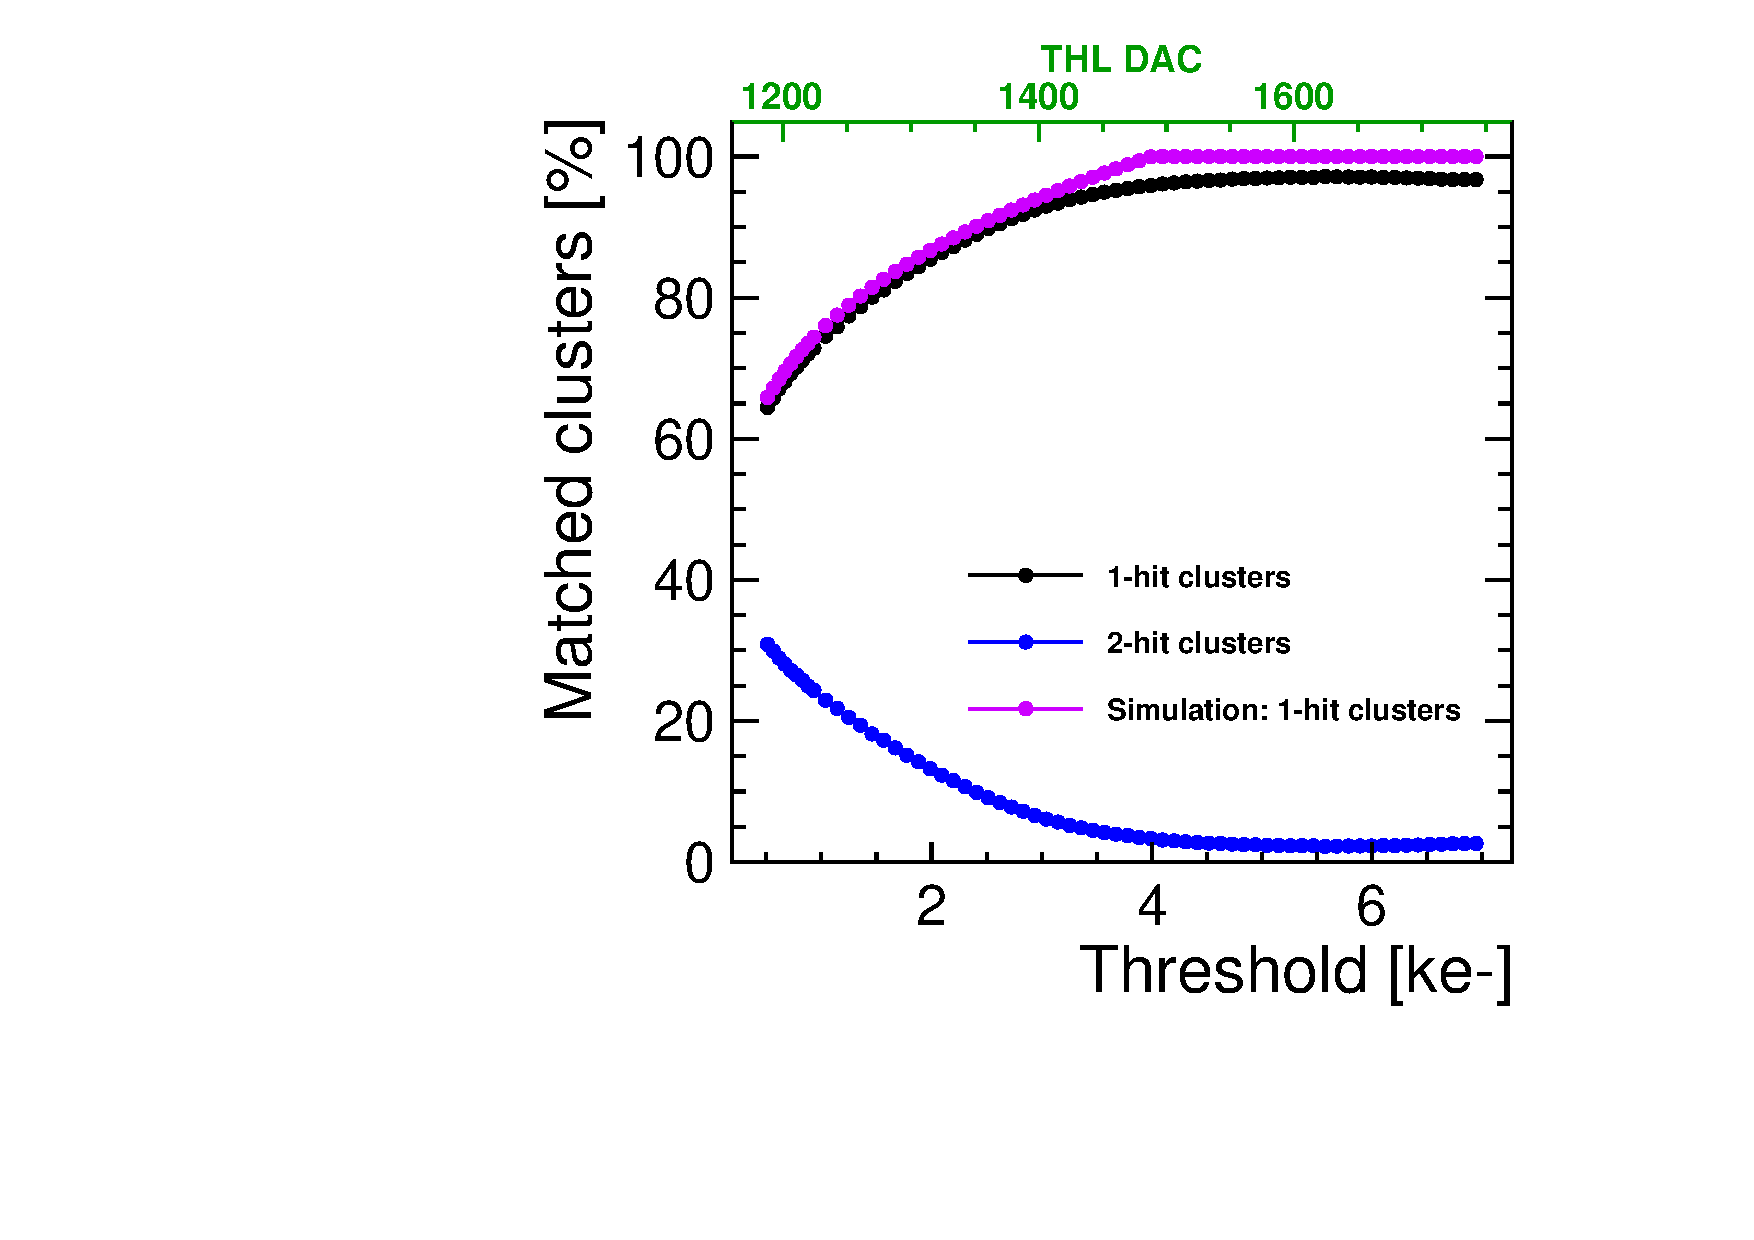
\includegraphics[width=\textwidth]{./figures/TestBeam/ThresholdScan_W0005_E02.pdf}
    \caption{}
  \end{subfigure} \hfill
  \begin{subfigure}[b]{0.45\textwidth}
%    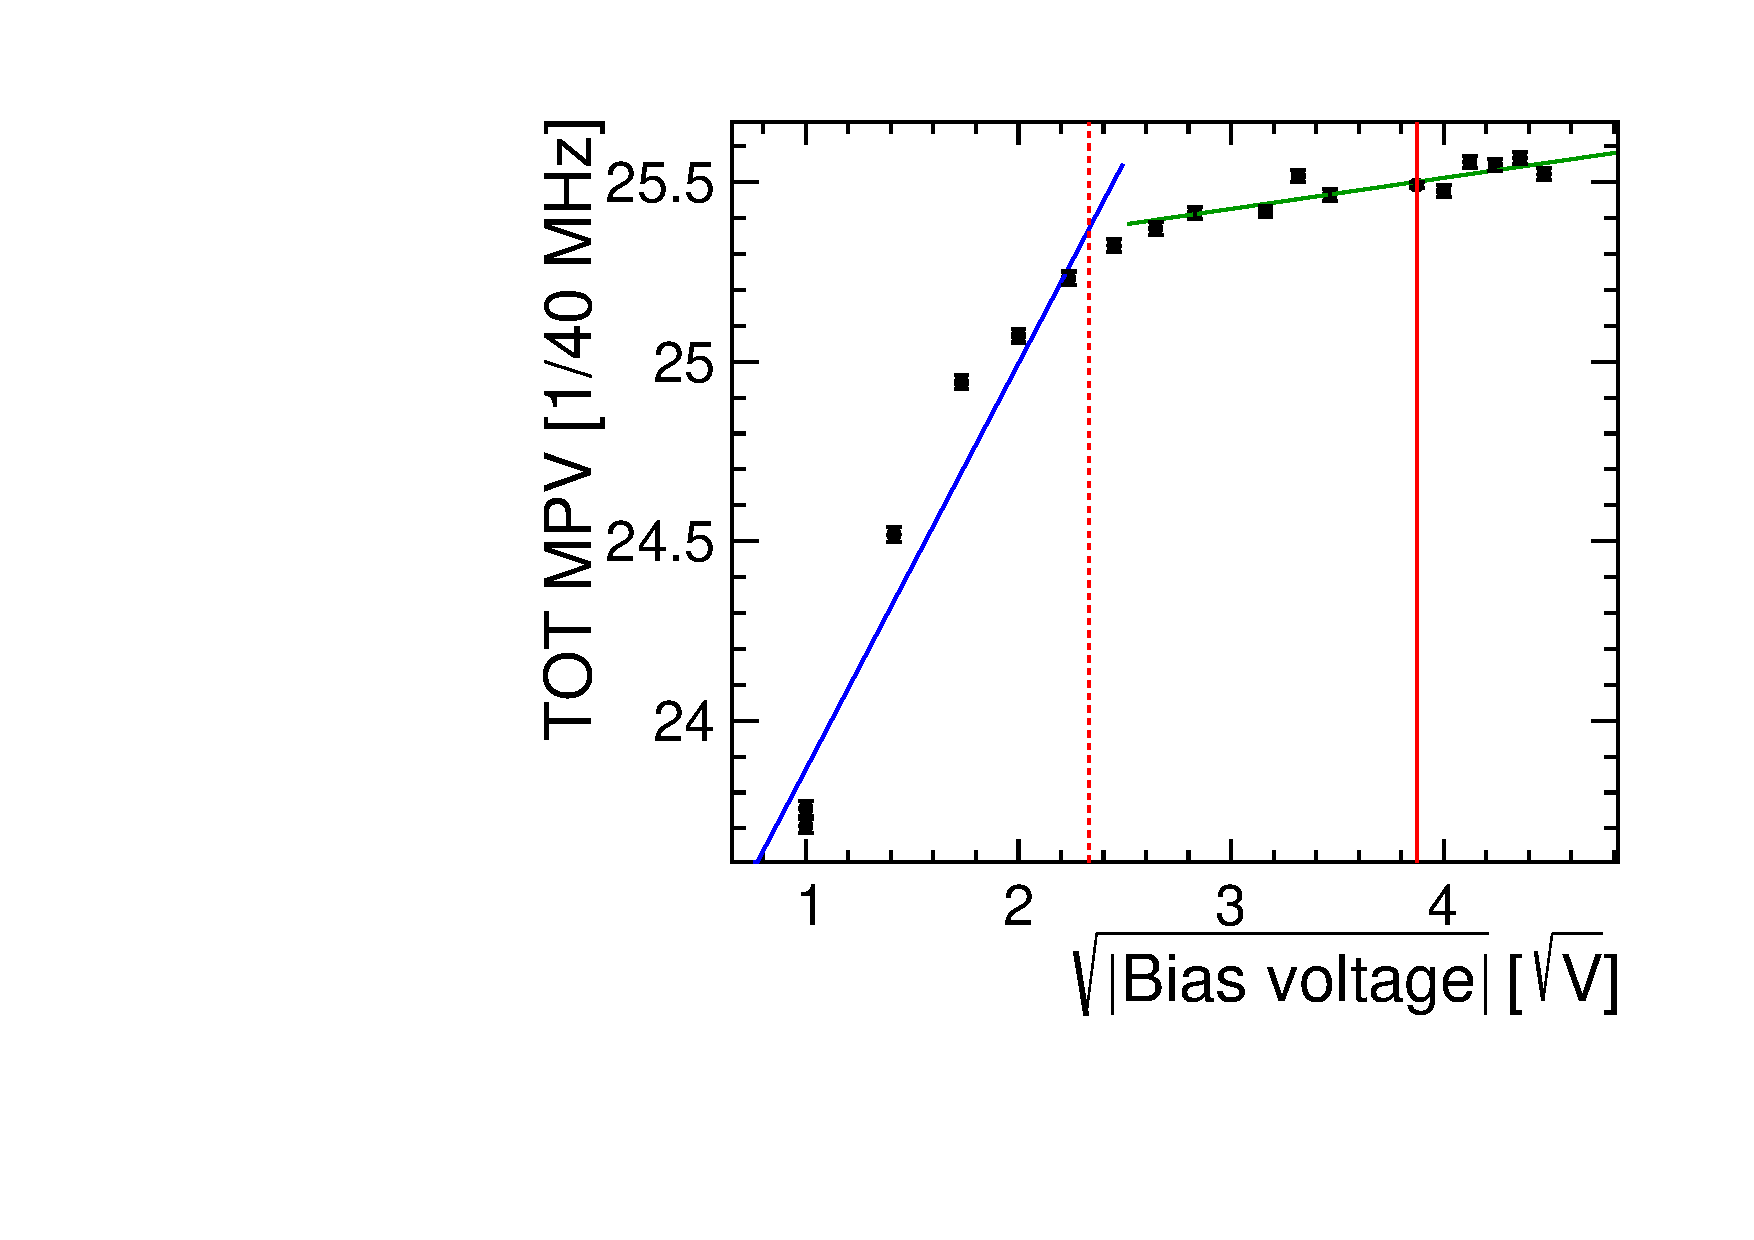
\includegraphics[width=\textwidth]{./figures/TestBeam/depletionVoltage_W0019_C07.pdf}
    \caption{}
  \end{subfigure}
  \caption{55-GNDGR-100 (W5\_E2): bias and voltage scan.}
  \label{fig:Timepix3_THLscan_Vdep_E2}
\end{figure}


\begin{figure}[htbp] \centering
  \begin{subfigure}[b]{0.45\textwidth}
    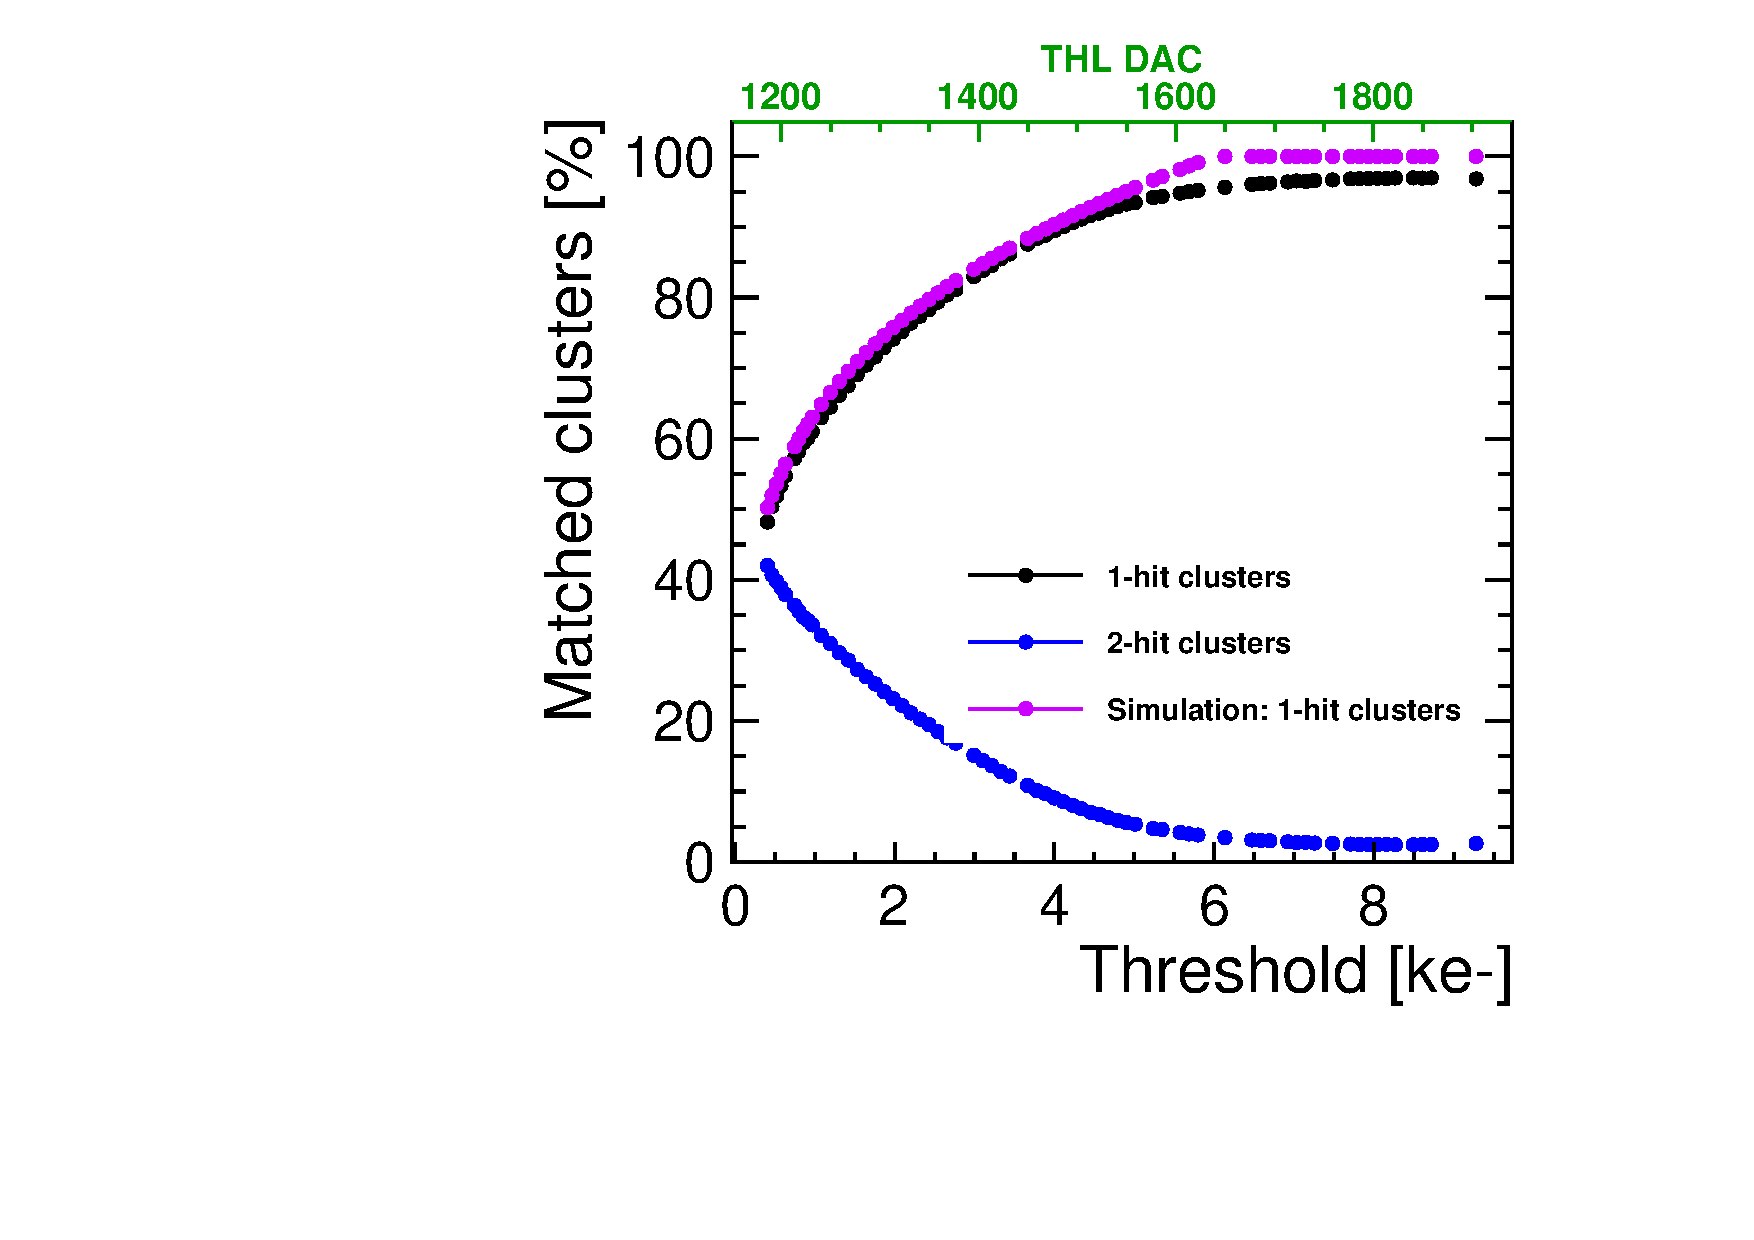
\includegraphics[width=\textwidth]{./figures/TestBeam/ThresholdScan_W0005_F01.pdf}
    \caption{}
  \end{subfigure} \hfill
  \begin{subfigure}[b]{0.45\textwidth}
    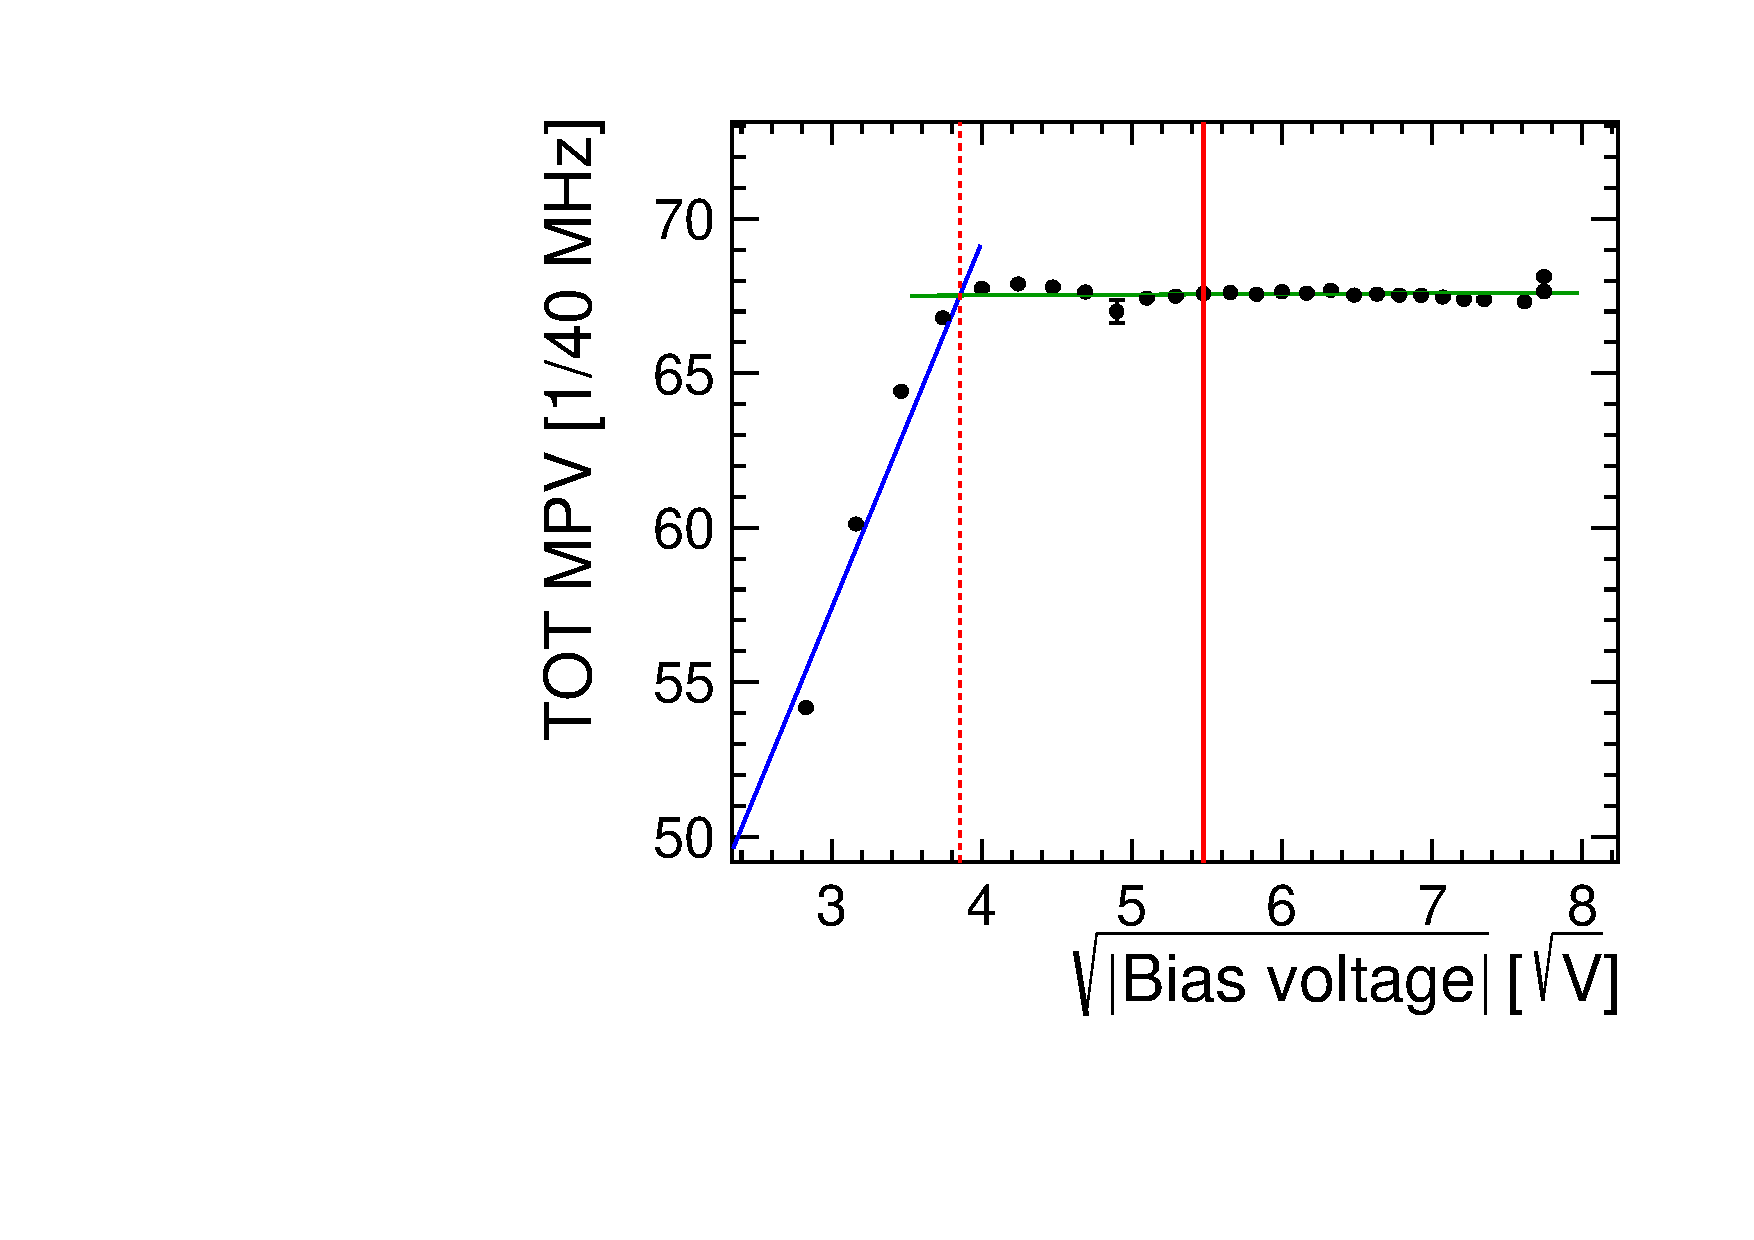
\includegraphics[width=\textwidth]{./figures/TestBeam/depletionVoltage_W0005_F01.pdf}
    \caption{}
  \end{subfigure}
  \caption{55-GNDGR-150 (W5\_F1): bias and voltage scan.}
  \label{fig:Timepix3_THLscan_Vdep_F1}
\end{figure}


%% --------------------------------------------- %%
\section{Validation of the simulation}
%% --------------------------------------------- %%
\section{Extrapolation to smaller pixels (CLICpix)}
